\section{Methods}
\label{sec:methods}

\subsection{Model Systems}

To assess the generality of evolutionary dynamics' effects on phylogenetic structure, we replicated experiments across models differing in subject and approach.
We used three systems,
\begin{enumerate}
\item a simple agent-based model with explicitly encoded fitness values;
\item Avida, a self-replicating agent-based evolutionary platform \citep{ofria2004avida}; and
\item Gen3sis, a population-level macro-ecological/evolutionary model \citep{hagen2021gen3sis}.
\end{enumerate}

The following introduces each model and details experiment-specific configurations.

\textbf{Simple Explicit-Fitness Model}


Experiments testing the relationships between evolutionary dynamics, reconstruction error, and phylogenetic structure required a model system amenable to direct, interpretable tuning of ecology, spatial structure, and selection pressure.
% @ELD: Maybe rename this section? I got through the first paragraph without realizing it was specifically about the simple modelAdditionally, in order to make findings relevant to large-scale phylogenetic analyses, computational efficiency was necessary to facilitate large population size and high generation counts.
Finally, a parsimonious and generic model system was desired so that findings would better generalize across digital evolution systems.
The core of this work relies on a simple agent-based model devised to fulfill these objectives.
% @ELD: Do we still want to say this is the core of the work now that we've got the other systems?
% @MAM: Depends how much of results the other parts end up taking up, I kind of imagine they might appear in a single section if they end up being similar to the simple model

Genomes in the explicit fitness model comprised a single floating-point value, with higher magnitude corresponding to higher fitness.
Population size 32,768 ($2^{15}$) was used for all experiments.
Selection was performed using tournament selection with synchronous generations.
Treatments' selection pressure was controlled via tournament size.
Mutation was applied after selection, with a value drawn from a unit Gaussian distribution added to all genomes.
Evolutionary runs were ended after 262,144 ($2^{18}$) generations.
Each run required around 4 hours of compute time.

Treatments incorporating spatial structure used a simple island model.
In spatially structured treatments, individuals were evenly divided among 1,024 islands and only competed in selection tournaments against sympatric population members.
Islands were arranged in a one-dimensional closed ring and 1\% of population members migrated to a neighboring island each generation.

Treatments incorporating ecology used a simple niche model.
Population slots were split evenly between niches.
Organisms were arbitrarily assigned to a niche at simulation startup and were only allowed to occupy population slots assigned to that niche.
Therefore, individuals exclusively participated in selection tournaments with members of their own niche.
In treatments also incorporating spatial structure, an even allotment of population slots was provided for every niche on every island.
Every generation, individuals swapped niches with probability $3.0517578125 \times 10^{-8}$ (chosen so one niche swap would be expected every 1,000 generations).

For our main experiments, we defined the following ``regimes'' of evolutionary conditions:
\begin{itemize}
  \item \textit{plain}: tournament size 2 with no niching and no islands,
  \item \textit{weak selection}: tournament size 1 with no niching and no islands,
  \item \textit{strong selection}: tournament size 4 with no niching and no islands,
  \item \textit{spatial structure}: tournament size 2 with no niching and 1,024 islands,
  \item \textit{weak ecology}: tournament size 2 with 4 niches and niche swap probability increased 100$\times$,
  \item \textit{ecology}: tournament size 2 with 4 niches, and
  \item \textit{rich ecology}: tournament size 2 with 8 niches.
\end{itemize}

In follow-up experiments testing ecological dynamics with a spatial background, we defined the following additional evolutionary ``regimes:''
\begin{itemize}
  \item \textit{plain}: tournament size 2 with no niching over 1,024 islands,
  \item \textit{weak ecology}: tournament size 2 with 4 niches and niche swap probability increased 100$\times$ over 1,024 islands,
  \item \textit{ecology}: tournament size 2 with 4 niches over 1,024 islands, and
  \item \textit{rich ecology}: tournament size 2 with 8 niches over 1,024 islands.
\end{itemize}

Finally, to foster generalizability of findings, all experiments were performed with two alternate ``sensitivity'' variables: evolutionary length in generations and mutation operator.
We saved phylogenetic snapshots at 32,768 generation epochs.
This allowed us to test shorter runs of 32,768 and 98,304 generations (through epochs 0 and 2) in addition to the full-length runs (through epoch 7).
One additional mutation operator was tested to contrast the unit Gaussian distribution: the unit exponential distribution.
Under this distribution, deleterious mutations are not possible and large-effect mutations are more likely.

Across all experiments, each treatment comprised 50 replicates.

\textbf{Avida Model}

Avida is a virtual agent-based model system used for sophisticated \textit{in silico} evolution experiments \citep{ofria2004avida}.
Notably, unlike the simple model described above, fitness within Avida arises implicitly from agents' self-replication activity, in relation to other agents' self-replication and the availability of shared exogenous resources.
Within Avida, digital organisms' genomes comprise a sequence of virtual CPU instructions.
Avida conducts open-ended evaluation of each agent's genetic program, affording the opportunity of copying itself into output memory and thereby creating an offspring agent.
Replication imposes an intrinsic baseline level of copy errors (i.e., mutations), ensuring an ongoing supply of genetic variation.
Because self-replicators compete for a limited quantity of population slots, Darwinian evolution ensues.
This scheme induces a complex fitness landscape, which is thought to better reflect the character of biological evolution \citep{adami2006digital}.

Under baseline conditions, Avidians compete on the basis of self-replication efficiency.
However, Avida may be configured to award extra CPU cycles to agents that complete boolean logic tasks.
To create the potential for multiple niches, we associated each task with a depletable resource.
Avidians only recieve CPU cycles for completeing a task if the corresponding resource is available, and completing a task depletes the associated resource.
Importantly, tasks can each be associated with different resources, or they can all be associated with the same resource.
Association of each task to an independent resource creates potential for stable ecological coexistence between task-specialized clades.
We added the constraint that Avidians may harvest at most two tasks with the intention of preventing generalists from disrupting task specialization.

Our baseline ``\textit{plain}'' treatment rewarded four boolean logic tasks (echo, not, nand, and), all drawing from a single resource with inflow rate 400 units per update.
Population structure was well-mixed and, to somewhat weaken the fecundity of high-fitness Avidians, replication destroyed the parent organism with probability 0.2.

We surveyed the following additional ``regimes'' of evolutionary conditions:
\begin{itemize}
  \item \textit{weak selection}: the probability of parent death was increased to 0.5;
  \item \textit{strong selection}: parent death probability was set to 0.0 and offspring were protected from replacement by their own offspring;
  \item \textit{spatial structure}: population was arranged as a two-dimensional toroidal grid, with Avidians replicating exclusively between neighboring population sites;
  \item \textit{weak ecology}: tasks were assigned independent resource pools, but three resources were only supplied at an inflow rate of 33 units while the fourth was supplied at 300 units per update,
  \item \textit{ecology}: each task drew from an independent resource pool with inflow rate of 100 units, and
  \item \textit{rich ecology}: 28 tasks were rewarded, each drawing from an independent resource pool with an inflow rate of 100 units.
\end{itemize}

In follow-up experiments, we defined the following additional evolutionary ``regimes'' with two-dimensional toroidal spatial struture,
\begin{itemize}
  \item \textit{plain}: four boolean logic tasks drawing from a single resource with inflow rate 400 units per update,
  \item \textit{weak ecology}: tasks were assigned independent resource pools, but three resources were only supplied at an inflow rate of 33 units while the fourth was supplied at 300 units per update,
  \item \textit{ecology}: each task drew from an independent resource pool with inflow rate of 100 units, and
  \item \textit{rich ecology}: 28 tasks were rewarded, each drawing from an independent resource pool with an inflow rate of 100 units.
\end{itemize}

\begin{figure*}
\begin{subfigure}[b]{1\columnwidth}
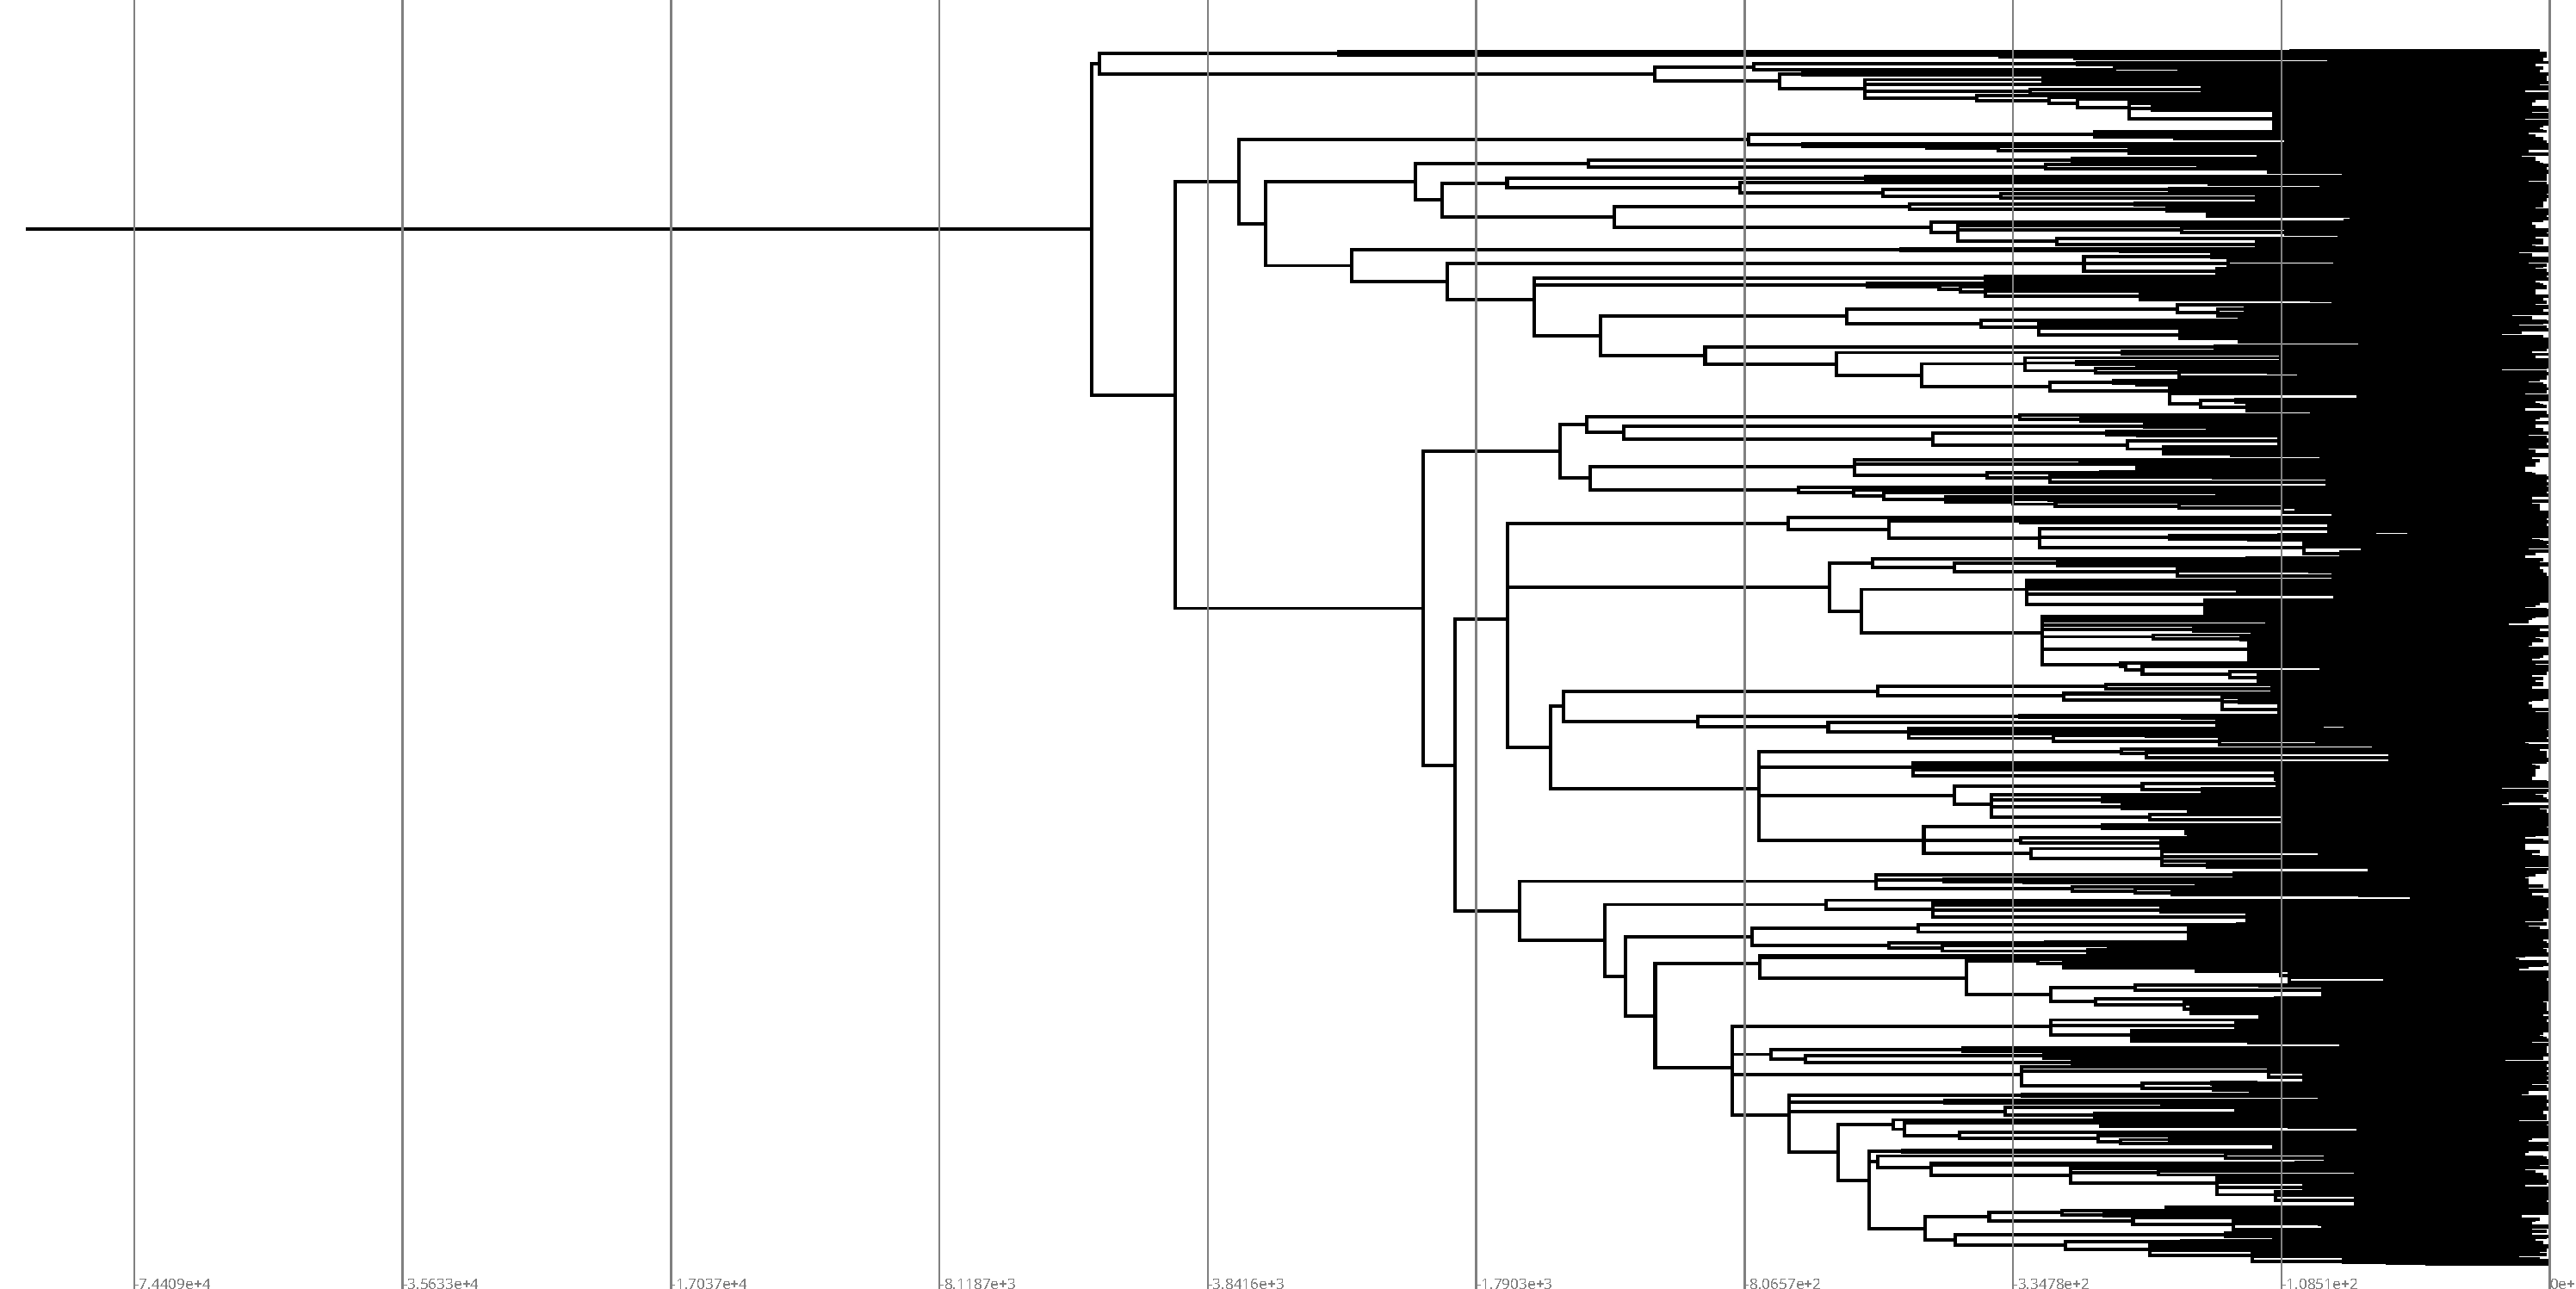
\includegraphics[height=0.12\textheight,width=\textwidth]{img/perfect-tree-phylogenies-log/avida-genome/model=avida+taxon=genome+treatment=plain+seed=1+phylogeny-snapshot-100000.pdf}
    % \end{noindent}
    \caption{%
      genome-level tracking}
    % \label{fig:perfect-tree-phylogenies-log:TODO}
  \end{subfigure}
  \hfill
  \begin{subfigure}[b]{1\columnwidth}
    % \begin{noindent}
    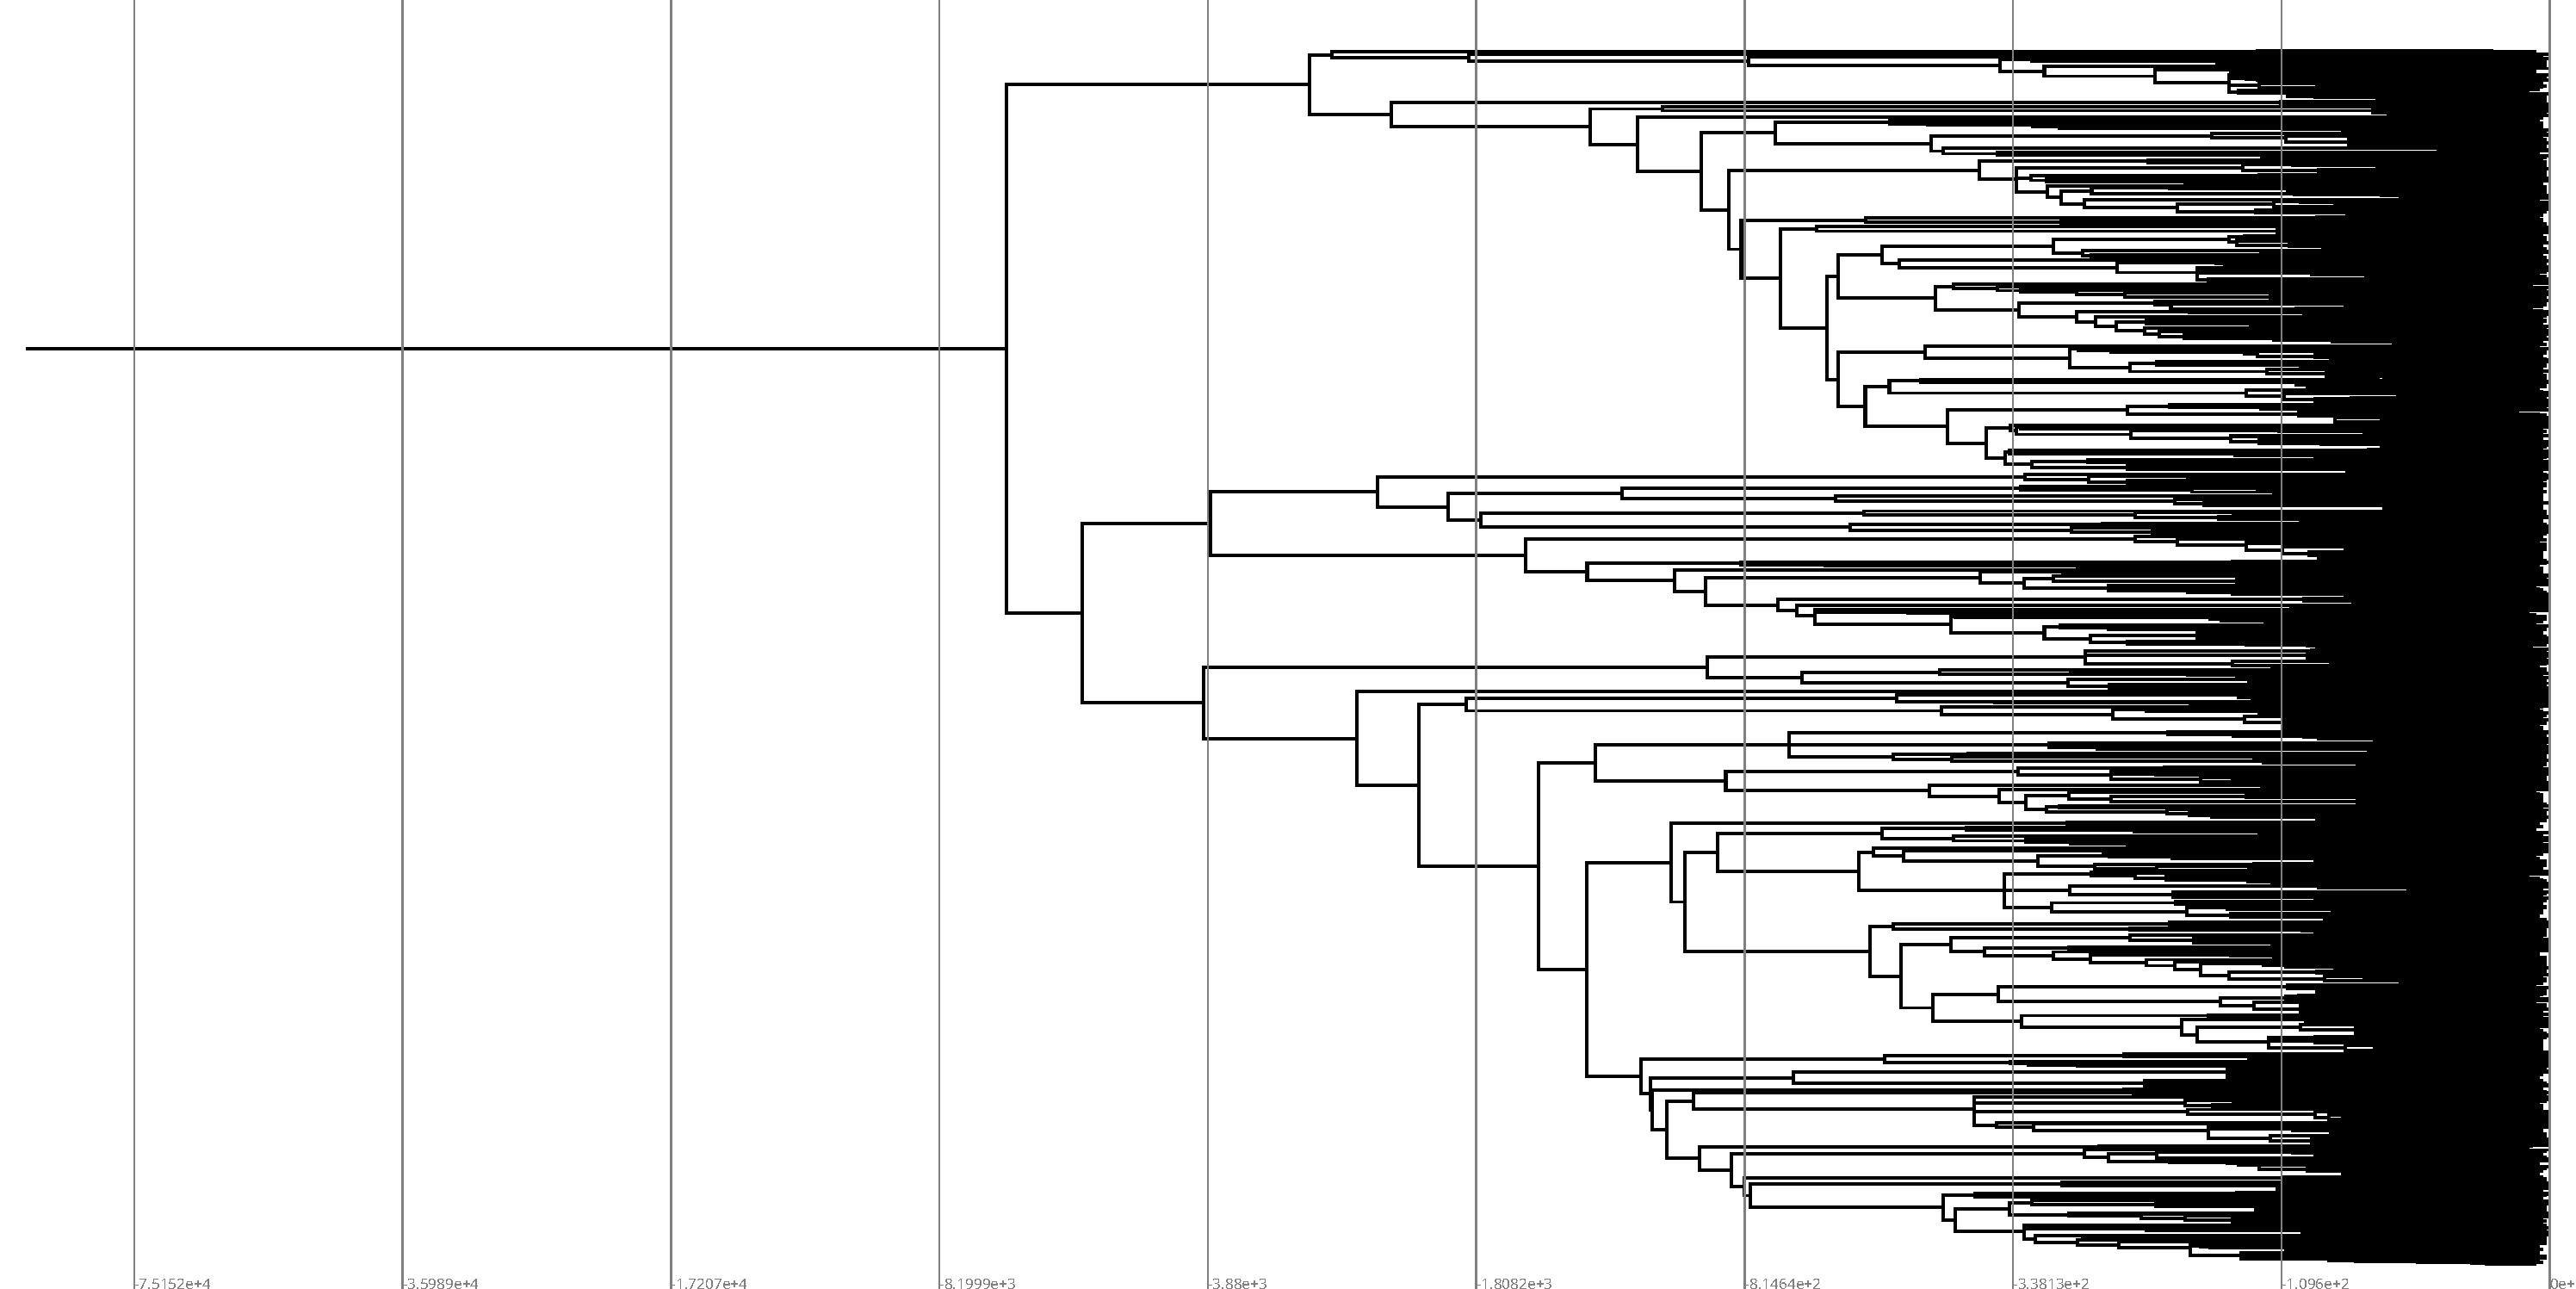
\includegraphics[height=0.12\textheight,width=\textwidth]{img/perfect-tree-phylogenies-log/avida-organism/model=avida+taxon=organism+treatment=plain_individual+seed=1+phylogeny-snapshot-100000.pdf}
    % \end{noindent}
    \caption{%
      organism-level tracking}
    % \label{fig:perfect-tree-phylogenies-log:TODO}
  \end{subfigure}
  \caption{%
    Sample reference phylogenies from Avida under ``plain'' regime.
    Time axis is log-scale.
  }
  \label{fig:perfect-tree-phylogenies-log-avida}
\end{figure*}


Experimental treatments using Avida comprised 30 replicates, conducted with population size 3,600 for durations of 100,000 time steps (c. 20k generations; range 9k-40k).
In order to achieve the phylogenetic tracking necessary for our experiments, we used a fork of Avida originally developed for research on MODES \citep{dolsonMODESToolboxMeasurements2019}, linked in supplemental materials described below.
This tracking system allowed two configurations: (1) tracking on the level of individual agents, where each Avidian constituted a taxonomic unit, or (2) tracking on the level of genotypes, where clonal sets of Avidians with identical genotypes constituted a taxonomic unit.
Figure \ref{fig:perfect-tree-phylogenies-log-avida} compares example phylogenies from Avida under the ``plain'' treatment, tracked at organism and genome level.
Surprisingly, we noticed several sign-change differences between individual-level and genotype-level tracking with respect to treatments' effects on phylometrics (Figures \ref{fig:perfect-tree-phylometrics-avida-heatmap} and \ref{fig:perfect-tree-phylometrics-heatmap-avida-genome}).
Much, but not all, of the difference related to effects of spatial structure.
These differences may be in part related to occurences of polytomies within genotype-level tracked phylogenies, as arbitrarily resolving polytomies into sets of bifurcating nodes gave somewhat more similar results to individual-level tracking.
Here, we report results from individual-level tracking, which corresponds to how phylogenies were tracked in the simple explicit-fitness model.

\textbf{Gen3sis Model}

In contrast to Avida and the simple fitness-explicit model, which are agent-based, Gen3sis is a population-level model.
Gen3sis abstracts evolution to interactions beetween spatially-dispersed, speciating subpopulations.
Co-located subpopulations of different species compete for shares of site-specific carrying capacity.
Interaction between subpopulation traits and environmental factors (e.g., aridity, temperature) mediates abundance determinations.
Disjoined subpopulations of the same species accumulate genetic incompatibilities absent sufficient gene flow and, past a defined incompatibility threshold, speciate.
Withhin this model, the taxonomic unit of phylogeny is species.

Gen3sis also stands out in its intended level of direct biological realism.
The software can be configured to reflect the particular geological and climate histories of continental biomes.
For our experiments, we used curated raster files depicting conditions over 30 million years in South America bundled with the package that had been synthesized from a number of sources \citep{straume2020global,westerhold2020astronomically,fick2017worldclim,hagen2019mountain,annan2013new,cramwinckel2018synchronous,evans2018eocene,hollis2019deepmip,hutchinson2018climate,keating2011warm,sijp2014role,zhang2019evolution}.

Among other features, Gen3sis allows differentiation of aquatic (e.g., lakes, ocean) zones from terrestrial regions with respect to suppression of inter-population migration rates.
To enhance potential for manipulable spatial structure within the model, we converted 30 randomly-selected thin linear segments spanning the map to be aquatic rather than terrestrial (i.e., ``rivers'').
Spatial structure was then induced by adjusting the water traversal cost function.

We assessed the following evolutionary regimes
\begin{itemize}
\item \textit{plain}: aquatic terrain imposed no additional migration penalties and population traits did not influence abundances,
\item \textit{spatial structure}: aquatic terrain imposed a migration barrier $50\times$ that of terrestrial terrain.
\item \textit{ecology}: species abundances were determined acccording to how close populations' trait value matches to site temperature,
\item \textit{ecology + spatial structure}: the $50\times$ aquatic dispersal penalty was applied and site temperature was used to determine species' abundances.
\end{itemize}
Figure \ref{fig:perfect-tree-phylogeny-gen3sis} shows an example Gen3sis phylogeny from the ``plain'' regime.

Gen3sis treatments comprised 30 replicates.
Note that, unlike other surveyed models, Gen3sis does not operate with constant ``population size.''
Rather, species count increased continuously over each of the 30 simulated 1 million year time steps as a consequence of ongoing speciation.
Maximum species count per spatial site was configured as 2,500 and within the entire simulation as 25,000, although neither limit was ever reached.

Full Gen3sis configuration files are linked in supplemental materials, described below.
For more on Gen3sis itself, see \citep{hagen2021gen3sis}.

\subsection{Hereditary Stratigraphic Annotations and Tree Reconstruction}

Experiments testing the impact of phylogenetic inference error on phylometrics employ the recently-developed ``hereditary stratigraphy'' technique to facilitate phylogenetic inference \citep{moreno2022hstrat}.
This technique works by attaching heritable annotations to individual digital genomes.
Every generation, a new random ``fingerprint'' is generated and appended to the individuals' inherited annotations.
To reconstruct phylogenetic history, fingerprints from extant organisms' annotations can be compared.
Where two organisms share identical fingerprints along the record, they likely shared common ancestry.
Mismatching fingerprints indicate a split in compared organisms' ancestry.
Although extensions of hereditary stratigraphy to sexual lineages are possible \citep{moreno2024methods}, all lineages used for experiments were asexual in nature.

Hereditary stratigraphy enables a tunable trade-off between annotation size and estimation accuracy.
Fingerprints may be discarded to decrease annotation size at the cost of reduced density of reference points to test for common (or divergent) ancestry along organisms' generational histories.

We test four levels of fingerprint retention.
Each level is described as a $p\%$ ``resolution'' meaning that the generational distance between reference points any number of generations $k$ back is less than $(p / 100) \times k$.
So, a high percentage $p$ indicates coarse resolution and a low percentage $p$ indicates fine resolution.
In detail, at the conclusion of 262,144 generation evolutionary runs,
\begin{itemize}
  \item at 33\% resolution 68 fingerprints are retained per genome,
  \item at 10\% resolution 170 fingerprints are retained per genome,
  \item at 3\% resolution 435 fingerprints are retained per genome, and
  \item at 1\% resolution 1,239 fingerprints are retained per genome.
\end{itemize}

This work uses 1 byte fingerprints, which collide with probability $1/256$.
Greater space efficiency could be achieved using 1 bit fingerprints.
However, this would require careful accounting for ubiquitous generation of identical fingerprints by chance and is left to future work.

Previous work with hereditary stratigraphy used UPGMA distance-based reconstruction techniques \citep{moreno2022hereditary}.
Large-scale reconstructions required for these experiments necessitated development of a more efficient technique that did not require all pairs (i.e., $O(n^2)$ distance comparison.
To accomplish this, we devised an agglomerative tree building algorithm that works by successively adding leaf organism annotations and percolating them down from the tree root along the tree path of internal nodes consistent with their fingerprint sequence, then affixing them where common ancestry ends.
This new tree-building approach reduced compute time from multiple hours to around 5 minutes in most cases.
Supplementary Listing \ref{lst:build_tree_trie} provides source code with full implementation details, see \citep{moreno2024analysis} for a more detailed discussion.

\begin{figure}
  \centering
  \begin{subfigure}[b]{\linewidth}
    \centering
    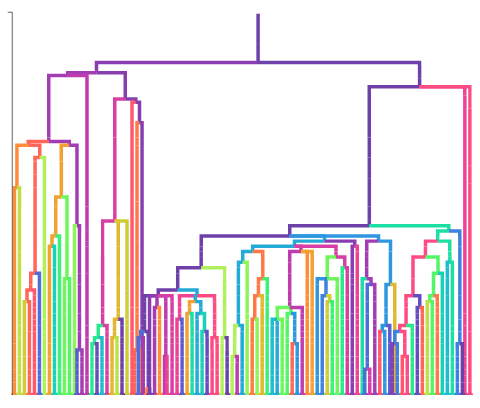
\includegraphics[width=\textwidth, height=0.13\textheight]{img/reference}
    \caption{%
      reference tree}
    \label{fig:plain-perfect-and-reconstruction-phylogenies:reference}
  \end{subfigure}
  \begin{subfigure}[b]{\linewidth}
    \centering
    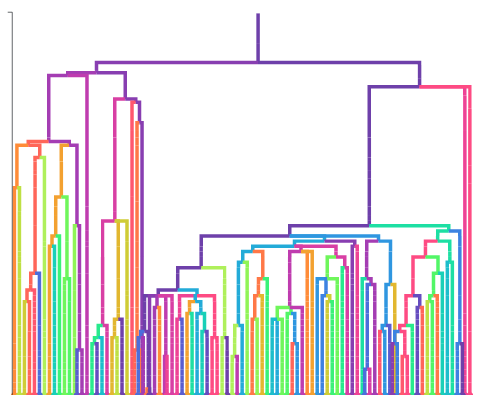
\includegraphics[width=\textwidth, height=0.13\textheight]{img/plain_resolution_100}
    \caption{%
      1\% resolution}
    \label{fig:plain-perfect-and-reconstruction-phylogenies:resolution_100}
  \end{subfigure}
  \begin{subfigure}[b]{\linewidth}
    \centering
    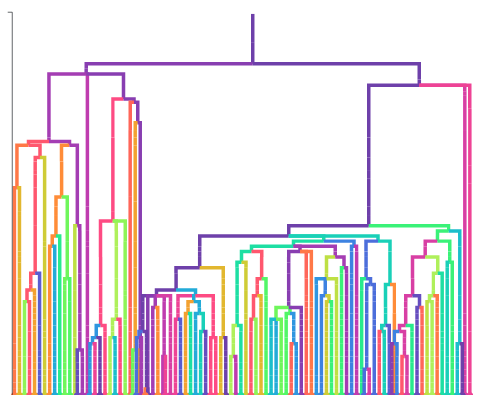
\includegraphics[width=\textwidth, height=0.13\textheight]{img/plain_resolution_30}
    \caption{%
      3\% resolution}
    \label{fig:plain-perfect-and-reconstruction-phylogenies:resolution_30}
  \end{subfigure}
  \begin{subfigure}[b]{\linewidth}
    \centering
    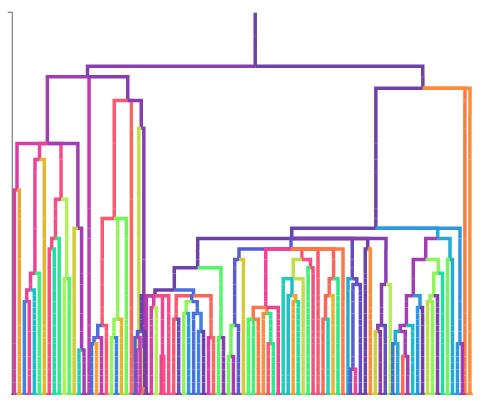
\includegraphics[width=\textwidth, height=0.13\textheight]{img/plain_resolution_10}
    \caption{%
      10\% resolution}
    \label{fig:plain-perfect-and-reconstruction-phylogenies:resolution_10}
  \end{subfigure}
  % \begin{noindent}
  \begin{subfigure}[b]{\linewidth}
    \centering
    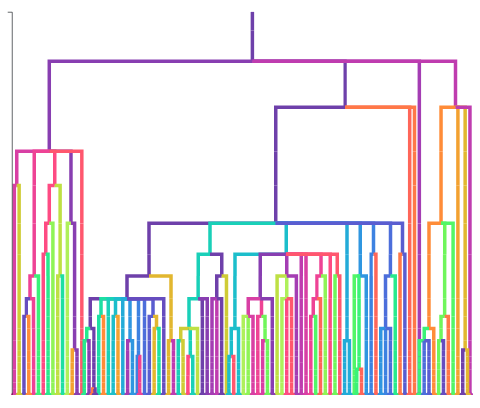
\includegraphics[width=\textwidth, height=0.13\textheight]{img/plain_resolution_3} \caption{%
      33\% resolution}
    \label{fig:plain-perfect-and-reconstruction-phylogenies:resolution_3}
  \end{subfigure}
  % \end{noindent}
  \caption{%
  \textbf{Comparison of phylogeny reconstructions across different hereditary stratigraphy resolutions in the plain evolutionary regime.}
    To maintain visual legibility, these trees contain the same sub-sample of 100 leaf nodes out of the 32,768 in the full trees.
    Sub-figures are arranged from top to bottom in coarsening order of reconstruction resolution.
    Taxon and branch color coding is consistent across subpanels.
    Visit \url{mmore500.com/hstrat-evolutionary-inference/} for mouseover-based highlighting of corresponding clades between reconstructions and reference.
  }
  \label{fig:plain-perfect-and-reconstruction-phylogenies}
\end{figure}


To assess the efficacy of the new agglomerative tree-building approach, we calculated all reconstructed trees' quartet distance to their respective reference.
Quartet distance ranges from 0 (between identical trees) to 0.75 (between random trees), providing in this case a measure of reconstruction error.
As expected, this measure of reconstruction error varied significantly with resolution for trees across all evolutionary regimes (Kruskal-Wallis tests; all $p < 10^{-20}$; Supplementary Table \ref{tab:reconstruction-error-comparisons-between-resolutions}).
Reconstruction error also varied significantly with evolutionary regime for each reconstruction resolution level (Kruskal-Wallis tests; all $p < 10^{-8}$; Supplementary Table \ref{tab:reconstruction-error-comparisons-between-regimes}).

For 3\% and 1\% resolutions, mean reconstruction error was less than 0.01 in all cases and at 10\% resolution mean reconstruction error was less than 0.05 in all cases.
At 33\% resolution, mean reconstruction error was less than 0.12 in all cases.
The largest reconstruction errors observed at 1\%, 3\%, 10\%, and 33\% resolutions were, respectively, 0.051 (weak selection regime), 0.093 (weak 4 niche ecology regime), 0.14 (plain evolutionary regime), and 0.45 (plain evolutionary regime).
Supplementary Table \ref{tab:tree-reconstruction-quality-quartet-summary-statistics} reports mean, median, standard deviation, and maxima for reconstruction error across surveyed evolutionary conditions.

To generate reconstructed trees in experiments, we simulated the inheritance of hereditary stratigraphic annotations along a reference phylogeny to yield the set of annotations that would be attached to extant population members at the end of a run, then used our agglomerative tree building technique to infer.
Thus, each reconstruction replicate has a directly-corresponding reference tree from a perfect-tree treatment replicate.
Figure \ref{fig:plain-perfect-and-reconstruction-phylogenies} shows a reference tree and corresponding reconstructions performed using 1\%, 3\%, 10\%, and 33\% resolution hereditary stratigraph annotations.

\subsection{Phylometrics}

A wide range of metrics exists for quantifying the topology of a phylogeny.
Tucker et. al showed that these metrics can be classified into the following three dimensions: richness, divergence, and regularity \citep{tuckerGuidePhylogeneticMetrics2017}.
Richness metrics quantify the amount of phylogenetic diversity/evolutionary history represented by a phylogeny.
Divergence metrics quantify how different the units of the phylogeny are from each other.
Regularity metrics quantify the variance of other properties (i.e. how consistent they are across the phylogeny).
Here, we focus on four metrics spread across these categories:

\textbf{Sum Pairwise Distance:} This measurement simply counts the total chronological length of lineages within the tree.
It is a metric of phylogenetic richness and is closely related to Faith's classic phylogenetic diversity metric \citep{faithConservationEvaluationPhylogenetic1992}.
Consequently, we would expect it to be increased by the presence of ecology or spatial structure, as both these factors increase diversity.
% TODO do we want to say more here?

\textbf{Colless-like Index:}
The original Colless Index \citep{collessReviewPhylogeneticsTheory1982}, also often referred to as $I_c$ \citep{shaoTreeBalance1990}, is a measure of tree imbalance (i.e., it gets higher as the tree gets less balanced).
In the context of Tucker et. al's framework, it is a regularity metric.
However, the traditional Colless Index only works for strictly bifurcating trees.
As our trees have multifurcations, we instead use the Colless-like Index, which is an extension of the Colless Index to multifurcating trees \citep{mirSoundCollesslikeBalance2018}.
Tree imbalance is thought to be associated with varying ecological pressures \citep{chamberlainPhylogeneticTreeShape2014, burressEcologicalOpportunityAlters} and has also been observed to increase in the presence of spatial structure \citep{scottInferringTumorProliferative2020}.

\textbf{Mean Pairwise Distance:}
This metric is calculated by computing the shortest distance between all pairs of leaf nodes and taking the mean of these values \citep{webbExploringPhylogeneticStructure2000}.
Note that these distances are measured in terms of the number of nodes in between the pair, not in terms of branch lengths.
Mean pairwise distance is a metric of evolutionary divergence \citep{tuckerGuidePhylogeneticMetrics2017}.
Mean pairwise distance should be increased by scenarios that promote the long-term maintenance of distinct phylogenetic branches, such as ecology.
Conversely, factors that act to reduce diversity should also reduce mean pairwise distance.

\textbf{Mean Evolutionary Distinctiveness:}
Evolutionary distinctiveness is a metric that can be calculated for individual taxa to quantify how evolutionarily different that taxon is from all other taxa in the phylogeny \citep{isaacMammalsEDGEConservation2007}.
To get mean evolutionary distinctiveness, we average this value across all extant taxa in the tree.
Like mean pairwise distance, mean evolutionary distinctiveness is a metric of evolutionary divergence.
However, it is known to capture substantially different information than mean pairwise distance \citep{tuckerGuidePhylogeneticMetrics2017}.
Unlike our other metrics, evolutionary distinctiveness is heavily influenced by branch length.
We generally expect mean evolutionary distinctiveness to be increased by similar factors to mean pairwise distance.

\subsection{Effect-size Analysis}

We expect statistical tests for between treatments we respect to evolutionary dynamics of interest to serve as an important use case for phylometric analyses in digital evolution.
As such, we wish to report the capability of reported phylometrics to discern betweensurveyed evolutionary conditions.

Cliff's delta provides useful nonparametric means for such effect size analysis.
This statistic reports the proportion of distributional non-overlap between two distributions, ranging from -1/1 if two distributions share no overlap to 0 if they overlap entirely \citep{meissel2024using,cliff1993dominance}.
When reporting effect size, we use conventional thresholds of 0.147, 0.33, and 0.474 to distinguish between negligible, small, medium, and large effect sizes \citep{hess2004robust}.

Note that the Cliff's delta statistic tops/bottoms out entirely once two distributions become completely separable.
Although this property suits most analyses performed, it is occasionally useful to distinguish the extent of divergence between phylometricc distributions past the point of complete seperability.
For these purposes, we perform a simple procedure to normalize phylometrics relative baseline conditions by subtracting out the baseline mean and dividingg by the baseline standardd deviation.

We typically pair effect-size analysis with Mann-Whitney U testing in order to assess the extent to which differences between phylometric readings under different conditions are, or are not, evidenced by ailable data \citep{mann1947on}.
As a final detail, note that we typically reort negated Cliff's delta values where necessary to ensure positive values correspond to larger phylometric vlaues and vice versa.

\subsection{Software and Data Availability}

Software, configuration files, and executable notebooks for this work are available at \url{https://github.com/mmore500/hstrat-evolutionary-inference}.
Data and supplemental materials are available via the Open Science Framework \url{https://osf.io/vtxwd/} \citep{foster2017open}.
Note that materials for earlier versions of this work are also contained in these repositories \citep{moreno2023toward}.

All hereditary stratigraph annotation, reference phylogeny generation, and phylogenetic reconstruction tools used in this work are published in the \texttt{hstrat} Python package \citep{moreno2022hstrat}.
This project can be visited at \url{https://github.com/mmore500/hstrat}.

This project uses data formats and tools associated with the ALife Data Standards project \citep{lalejini2019data} and benefited from many pieces of open-source scientific software \citep{ofria2020empirical,sand2014tqdist,2020SciPy-NMeth,harris2020array,reback2020pandas,mckinney-proc-scipy-2010,sukumaran2010dendropy,cock2009biopython,dolson2024phylotrackpy,torchiano2016effsize,waskom2021seaborn,hunter2007matplotlib,moreno2024apc,moreno2024qspool,moreno2023teeplot,hagen2021gen3sis,ofria2004avida,torchiano2016effsize}.